\subsection{Variabilidade de documentos recomendados}

Outro fator interessante de analisar é a variabilidade de documentos recomendados ao variar os parâmetros de treinamento. No conjunto de resultados cada documento 
de origem tem \textbf{336 valores}, número este que vem da combinação de valores possíves das variações dos parâmetros número de tópicos,
\textit{alpha}, \textit{eta}, \textit{passes} e de 2 conjuntos de páginas diferentes.

Agrupando por documento de origem eu contei a quantidade de documentos destinos diferentes que foram recomendados como o mais semelhante e abaixo
está a lista ordenada contendo os 5 com menor variação e os 5 com maior.

No geral o documento com \textit{id} 7923 teve 43 documentos de destino recomendados com o mais semelhante. Isto quer dizer que o post do blog com 
este \textit{id} teve 43 páginas na Wikipedia recomendadas como a mais parecida entre as 336 comparações realizadas para este documento no total.

No outro extremo temos o documento de origem com \textit{id} 6798, que teve 168 documentos distintos recomendados para este documento. Isto
quer dizer que a variação nos parâmetros influenciou muito na identificação de semelhança para este documento.

\begin{center}
    \begin{tabular}{|c|c|}
        \hline
        \textbf{Id do documento de origem} & \textbf{Documentos destino diferentes} \\
        \hline
        7923 & 43 \\
        \hline
        7131 & 45 \\
        \hline
        8116 & 46 \\
        \hline
        7108 & 48 \\
        \hline
        8146 & 51 \\
        \hline
        ... & ... \\
        \hline
        8896 & 157 \\
        \hline
        5641 & 158 \\
        \hline
        134 & 158 \\
        \hline
        3721 & 158 \\
        \hline
        6798 & 168 \\
        \hline
    \end{tabular}
\end{center}

O gráfico a seguir mostra a distribuição da quantidade de documentos distintos por documento de origem. Notamos que a maior concentração
de documentos semelhantes distintos recomendados por origem está perto de 120.

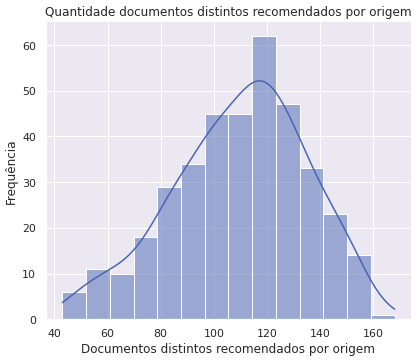
\includegraphics[scale=0.7]{resultados/resources/distribuicao_semelhantes_distintos.png}

Vamos então ver como esta variabilidade é influenciada pelos parâmetros de treinamento do algoritmo para entender quais tem maior peso.

Começando pelo número de tópicos, vamos ver os 5 que mais se destacam nos dois extremos, os que têm maior e menor variação. Cada combinação de 
documento de origem e número de tópicos aparece 48 vezes no resultado (3 \textit{alpha} * 4 \textit{eta} * 2 \textit{passes} * 2 \textit{cenario\_wp}).

O documento de \textit{id} 5599 se mostrou o que menos é influenciado pela variação dos demais parâmetros quando o número de tópicos foi
\textit{39}, tendo apenas 4 documentos distintos recomendados nos 48 resultados para esta combinação.

No outro extremo temos o documento com \textit{id} 8896, que teve com 67 tópicos teve 38 recomendações distintas, uma variação muito grande.

\begin{center}
    \begin{tabular}{|c|c|c|}
        \hline
        \textbf{Id do documento de origem} & \textbf{Número de tópicos} & \textbf{Documentos destino diferentes} \\
        \hline
        5599 & 39 & 4 \\
        \hline
        14565 & 22 & 7 \\
        \hline
        5599 & 57 & 7 \\
        \hline
        14565 & 39 & 8 \\
        \hline
        13988 & 39 & 8 \\
        \hline
        ... & ... & ... \\
        \hline
        10475 & 72 & 36 \\
        \hline
        8896 & 57 & 36 \\
        \hline
        10399 & 101 & 36 \\
        \hline
        14946 & 45 & 37 \\
        \hline
        8896 & 67 & 38 \\
        \hline
    \end{tabular}
\end{center}

Vamos ver agora a distribuição gráfica destes valores recomendados por tópico.

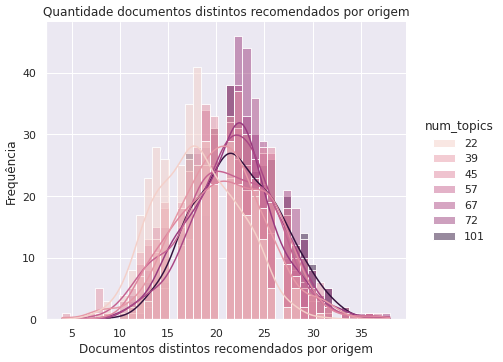
\includegraphics[scale=0.7]{resultados/resources/distribuicao_semelhantes_distintos_topics.png}

Em seguida vemos os 5 que mais se destacam nos dois extremos em relação ao parâmetro \textit{alpha}, os que têm maior e menor variação. 
Cada combinação de documento de origem e valor de alpha aparece 112 vezes no resultado (7 \textit{num\_topics} * 4 \textit{eta} * 2 \textit{passes} * 2 \textit{cenario\_wp}).

Assim como na comparação por tópicos, o documento de \textit{id} 5599 se mostrou o que menos é influenciado pela variação dos demais 
parâmetros quando o valor alpha \textit{1.00}, tendo apenas 5 documentos distintos recomendados nos 112 resultados para esta combinação.

No outro extremo temos o documento com \textit{id} 6798, que teve com valor \textit{alpha} 0.10 teve 77 recomendações distintas.

\begin{center}
    \begin{tabular}{|c|c|c|}
        \hline
        \textbf{Id do documento de origem} & \textbf{Alpha} & \textbf{Documentos destino diferentes} \\
        \hline
        5599 & 1.00 & 5 \\
        \hline
        13617 & 1.00 & 8 \\
        \hline
        13360 & 1.00 & 9 \\
        \hline
        13356 & 1.00 & 10 \\
        \hline
        15389 & 1.00 & 11 \\
        \hline
        ... & ... & ... \\
        \hline
        8896 & 0.10 & 76 \\
        \hline
        6637 & 0.10 & 76 \\
        \hline
        14946 & 0.01 & 77 \\
        \hline
        8896 & 0.01 & 77 \\
        \hline
        6798 & 0.10 & 77 \\
        \hline
    \end{tabular}
\end{center}

O gráfico abaixo nos mostra que ao utilizar valor \textit{alpha} 1.0 a tendência é que a quantidade de documentos distintos recomendados por 
documento de origem seja muito menor, causando menor variabilidade. Lembrando que este valor mais alto indica pro algoritmo que mais tópicos definem 
os contextos dos textos. Para valores \textit{alpha} 0.1 e 0.01 a variabilidade é maior mas com pouca diferença entre um e outro na distribuição.

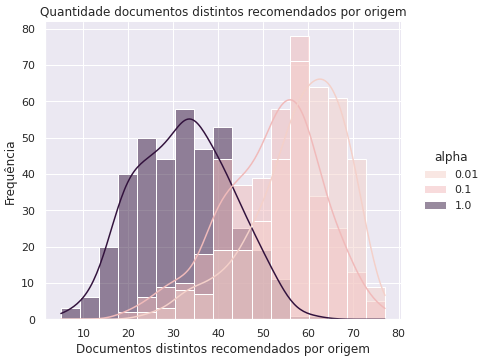
\includegraphics[scale=0.7]{resultados/resources/distribuicao_semelhantes_distintos_alpha.png}

O próximo parâmetro analisado é o \textit{eta}, onde também analisamos os 5 que mais se destacam nos dois extremos em relação ao parâmetro.
Cada combinação de documento de origem e valor de \textit{eta} aparece 84 vezes no resultado (7 \textit{num\_topics} * 3 \textit{alpha} * 2 \textit{passes} * 2 \textit{cenario\_wp}).

Aqui o documento com menor variação é o com \textit{id} 3339, que para o valor \textit{eta} 0.005 teve apenas 15 documentos distintos. Nota-se aqui
que mesmo não sendo o que mais se destaca houve também pouca variação para o documento com \textit{id} 5599.
No outro extremo temos o documento com \textit{id} 5641, que teve com valor \textit{eta} 0.005 teve 61 recomendações distintas, o que é um número 
grande comparado com as 84 execuções para este par.

\begin{center}
    \begin{tabular}{|c|c|c|}
        \hline
        \textbf{Id do documento de origem} & \textbf{Eta} & \textbf{Documentos destino diferentes} \\
        \hline
        3339 & 0.005 & 15 \\
        \hline
        15389 & 0.005 & 15 \\
        \hline
        5599 & 0.050 & 15 \\
        \hline
        7185 & 1.000 & 16 \\
        \hline
        13870 & 0.050 & 16 \\
        \hline
        ... & ... & ... \\
        \hline
        8896 & 0.005 & 57 \\
        \hline
        6798 & 0.005 & 58 \\
        \hline
        8896 & 1.000 & 58 \\
        \hline
        14946 & 0.500 & 59 \\
        \hline
        5641 & 0.005 & 61 \\
        \hline
    \end{tabular}
\end{center}

A distribuição abaixo nos mostra que a maior concentração de documentos distintos é semelhante para qualquer valor de \textit{eta}, perto da faixa de 
35 documentos. A diferença acontece na quantidade de valores nesta faixa, que aumenta quando se aumenta o \textit{eta} e na faixa com maior 
quantidade de documentos distintos um valor mais baixo do parâmetro se destaca, com maior concentração).

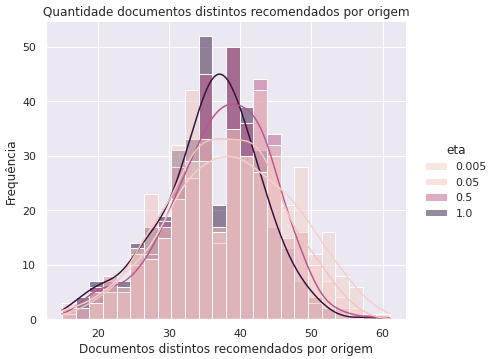
\includegraphics[scale=0.7]{resultados/resources/distribuicao_semelhantes_distintos_eta.png}

O próximo parâmetro analisado é o \textit{passes}, onde abaixo analisamos os 5 que mais se destacam nos dois extremos em relação ao parâmetro.
Cada combinação de documento de origem e valor de \textit{eta} aparece 168 vezes no resultado (7 \textit{num\_topics} * 3 \textit{alpha} * 4 \textit{eta} * 2 \textit{cenario\_wp}).

Aqui o documento com menor variação novamente é o com \textit{id} 5599, que para o valor de \textit{passes} 2 teve apenas 26 documentos distintos. 
No outro extremo temos o documento com \textit{id} 3326, que com valor de \textit{passes} 10 teve 102 recomendações distintas.

\begin{center}
    \begin{tabular}{|c|c|c|}
        \hline
        \textbf{Id do documento de origem} & \textbf{Passes} & \textbf{Documentos destino diferentes} \\
        \hline
        5599 & 2 & 26 \\
        \hline
        7923 & 27 & \\
        \hline
        7131 & 10 & 27 \\
        \hline
        7108 & 10 & 29 \\
        \hline
        8116 & 10 & 30 \\
        \hline
        ... & ... & ... \\
        \hline
        6766 & 10 & 94 \\
        \hline
        6798 & 10 & 95 \\
        \hline
        8018 & 10 & 96 \\
        \hline
        8896 & 2 & 100 \\
        \hline
        3326 & 10 & 102 \\
        \hline
    \end{tabular}
\end{center}

A análise gráfica abaixo nos mostra que apesar de ter uma diferença na concentração na faixa com maior frequência, a variação para este parâmetro 
não se mostrou muito significativa.

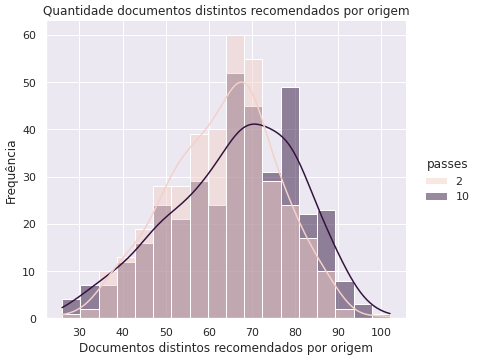
\includegraphics[scale=0.7]{resultados/resources/distribuicao_semelhantes_distintos_passes.png}

Em seguidas analisamos os extremos de variação ao limitar o tamanho dos documentos utilizados na comparação.
Assim como no caso anterior, cada combinação de documento de origem e cenário Wikipedia aparece 168 vezes no resultado (7 \textit{num\_topics} * 3 \textit{alpha} * 4 \textit{eta} * 2 \textit{passes}).

Aqui o documento com menor variação novamente é o com \textit{id} 8116, que para a base de comparação reduzida teve apenas 21 documentos distintos. 
No outro extremo temos o documento com \textit{id} 6798, que na base de comparação completa 125 recomendações distintas.

Um fato interessante a se notar é que os 5 que menos variam ocorreram na base reduzida, enquanto os 5 maiores aparecem na base de comparação completa.

\begin{center}
    \begin{tabular}{|c|c|c|}
        \hline
        \textbf{Id do documento de origem} & \textbf{cenario\_wp} & \textbf{Documentos destino diferentes} \\
        \hline
        8116 & gte42 & 21 \\
        \hline
        7131 & gte42 & 21 \\
        \hline
        7923 & gte42 & 24 \\
        \hline
        7344 & gte42 & 24 \\
        \hline
        7108 & gte42 & 25 \\
        \hline
        ... & ... & ... \\
        \hline
        5232 & full & 118 \\
        \hline
        5093 & full & 118 \\
        \hline
        3326 & full & 120 \\
        \hline
        8377 & full & 122 \\
        \hline
        6798 & full & 125 \\
        \hline
    \end{tabular}
\end{center}

A análise gráfica abaixo nos mostra que ao excluir da comparação documentos com pouca quantidade de tokens a variação na quantidade de documentos
distintos recomendados por documento de origem dimimui. Por aqui nota-se o mesmo que percebemos na tabela acima, que é a predominância da base reduzida
no extremos de menor variação e da base completa na área de maior variação. Isto mostra uma tendência do algoritmo em "ter mais dúvidas" quando usamos 
a base completa. Mas a diferença neste caso não ocorre por somente por causa do tamanho dos documentos, há também a diminuição nas opções disponíveis para
comparação.

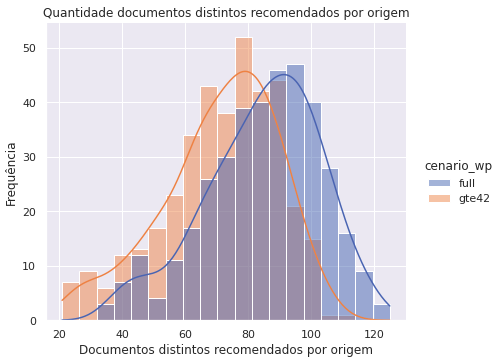
\includegraphics[scale=0.7]{resultados/resources/distribuicao_semelhantes_distintos_cenario_wp.png}

